\chapter{Sissejuhatus}\label{chapter:introduction}
Foneetikauuringutes kasutatakse kõnekorpusi, mis sisaldavad sadade inimeste kõnenäiteid. Korpuste analüüsil leitakse erinevaid akustilisi tunnuseid, nagu põhitoon (F0), formandid, spektrid ja muud hääle kvaliteeti kirjeldavad tunnused. Nende tunnuste abil saab tuvastada erinevaid kõnestiile, võõrkeele aktsente, emotsionaalseid ja tervislikke seisundeid.

Üheks laialt levinud tunnustekomplektiks foneetikauuringutes on GeMAPS (The Geneva Minimalistic Acoustic Parameter Set) \cite{eyben2016gemaps}. See komplekt sisaldab mitmeid olulisi akustilisi tunnuseid, mida saab kasutada mitmesugustes uuringutes. Paraku ei ole hetkel kuigi palju tööriistu, mis võimaldaksid GeMAPS-tunnuste automaatset helisalvestisest eraldamist ja põhjalikumat visualiseerimist ühes rakenduses.

Korpuste analüüsi tööprotsessi osad on sageli järgmised tegevused: akustiliste tunnuste eraldamine kõnefailidest, akustiliste tunnuste visualiseerimine, uurija poolt etteantud akustiliste omadustega kõnenäidete leidmine. Kuigi on olemas mitmeid tööriistu, mis suudavad neid ülesandeid eraldi täita, puudub hetkel terviklik rakendus, mis võimaldaks täita kõiki neid kõnekorpuste analüüsiga seotud ülesandeid.

Selle bakalaureusetöö eesmärk on luua tööriist, mis võimaldab:
\begin{itemize}
    \item GeMAPS tunnuste eraldamist kõnefailidest,
    \item tunnuste visualiseerimist erinevatel diagrammitüüpidel: joondiagramm ajateljel, vokaalikaart, radar, karpdiagramm ja histogramm,
    \item sarnaste kõnelejate otsingut ja kõnekorpusest.
\end{itemize}

Loodud rakendus on abiks uurijatele, kes soovivad kasutada GeMAPS-tunnuseid foneetika- või hääleanalüüsis. Rakendus koondab mitmed peamised uurimisprotsessi funktsioonid nagu: tunnuste eraldamine, andmete visualiseerimine ja sarnaste salvestiste leidmine.


\chapter{Olemasolevad rakendused}\label{chapter:taust}
Järgnevalt antakse lühike ülevaade sarnase funktsionaalsusega olemasolevatest kõneanalüüsi tööriistadest. 

\textbf{Kõneveebi Audiofailide akustiliste omaduste võrdlus} \cite{kõneveeb} on veebirakendus, mis kasutab OpenSMILE eGeMAPS tunnuste komplekti kõnesalvestiste akustiliseks analüüsiks.

Rakenduse võimalused:
\begin{itemize}
    \item .wav-formaadis pakendatud audiofailide üleslaadimine, maksimaalne lubatud failide suurus 900MB
    \item Võimalik määrata klassifikaatoreid CSV-vormingus.
    \item Visualiseeritakse valitud akustiliste tunnuste väärtuste jaotus joondiagrammina
    \item Arvutatud väärtused ja üleslaetud failid kustutatakse peale brauseri sulgemist.
\end{itemize} 

\textbf{Praat} \cite{praat} on Amsterdami Ülikoolis arendatud vabavaraline kõneanalüüsi rakendus ning väga levinud foneetikauuringutes. Praat toetab Windows, macOS ja Linux operatsioonisüsteeme.
 
Rakenduse võimalused:
\begin{itemize}
    \item Akustiline analüüs ja erinevate tunnuste arvutamine (F0, formandid, intensiivsus, jitter, shimmer jpm)
    \item Visualiseerimisvõimalused: spektrogrammid, põhitooni ja intensiivsuse graafikud ajateljel, formantide trajektoorid
    \item Kõnesüntees: põhitooni ja formantide põhjal on võimalik luua modifitseeritud või sünteesitud kõne
    \item Skriptide loomise võimalus: Praatil on oma skriptikeel, mis teeb rakenduse paindlikuks, ning võimaldab automatiseerida korduvaid analüüse
\end{itemize}

\textbf{VoiceSauce} \cite{voicesauce} on MATLAB-i keskkonnas arendatud kõneanalüüsi rakendus. Rakendus on mõeldud teaduslikuks kõneanalüüsiks. Toetatud on Windows ja macOS operatsioonisüsteemid.

Rakenduse võimalused:
\begin{itemize}
    \item Erinevate akustiliste hääle tunnuste visualiseerimine ja analüüs.
    \item Mõned parameetrid sõltuvad tugevalt arvutatud F0 väärtustest, mistõttu võib analüüs olla ebatäpne mürarikaste helide korral
    \item Pikkade heliklippide analüüs võib tekitada ressursipuudust, kuna MATLABi keskkond võib intensiivsel analüüsil väga suurt osa mälu tarbida.
    \item Nõuab MATLABi kasutamist
\end{itemize} 

\textbf{Wasp (Windows Tool for Speech Analysis)} \cite{wasp} on tasuta kõneanalüüsi rakendus. Toetatud on operatsioonisüsteem Windows.

Rakenduse võimalused:
\begin{itemize}
    \item Helifailide salvestamine ja esitamine, salvestatud faile on võimalik analüüsida
    \item Võimaldab luua annotatsioone
    \item Akustiliste tunnuste visualiseerimine
    \item Lihtne ja kasutajasõbralik kasutajaliides ning saadaval on veebiversioon rakendusega tutvumiseks
\end{itemize} 

Kõik välja toodud rakendused (Kõneveebi veebirakendus, Praat, VoiceSauce ja Wasp) on võimelised kõnesalvestusi töötlema ning pakuvad akustiliste tunnuste arvutamist ja visualiseerimisvõimalusi. Neist kõige rohkem võimalusi ja funktsionaalsust on Praatil, kuid sellel ei ole spetsiaalset funktsionaalsust GeMAPS tunnuste eraldamiseks. Samuti on erinevate visualisatsioonide ja analüüside jaoks tavaliselt vajalik skriptide kirjutamine.

Selgelt erinev teistest on Kõneveebi lahendus, sest see on veebipõhine ning mõeldud ainult eGeMAPS-tunnuste analüüsiks. Selle funktsionaalsus on piiratud: rakenduses on küll võimalik akustilisi tunnuseid joondiagrammil visualiseerida, kuid puuduvad erinevad diagrammitüübid ning analüüsimeetodid sarnasuse otsinguks. Lisaks esineb failisuuruse piirang ja tulemusi ei salvestata.

Seega, ükski rakendus ei kata ühes keskkonnas kõiki käesolevas töös esile toodud analüüsiülesandeid: GeMAPS tunnuse arvutamine, erinevad visualiseerimis võimalused ning sarnasuse analüüsi.


\chapter{Rakenduse nõuded}\label{chapter:nõuded}
\input{chapters/3. Rakenduse nõuded}

\chapter{Rakenduse arendus}\label{chapter:arendus}
\section{Tunnuste eraldamine ja TextGridide töötlus}
Järgnevalt kirjeldatakse akustiliste tunnuste helifailist eraldamise protsessi ja ktehnoloogiaid. Ning TextGridide töötlemiseprotsessi ja tehnoloogiaid

\subsection{OpenSMILE}
Tunnuste eraldamise protsess: sisendiks on helifail -> opensmile töötleb -> väljund pandas DataFrame tunnustega, mis on eraldatud iga salvestuse 10ms ajahetke kohta.

Konfiguratsioonis määratakse tunnuste komplekt - neid on mitmeid erinevaid. Rakenduses kasutatakse kõige väiksemat eGeMAPS v02 akustiliste tunnuste komplekti, kus on 88 tunnust, mis jagunevad:

\begin{enumerate}
    \item Madala taseme deskriptorid (LLD): otseselt helisignaalist tuletatud tunnused
    \item Funktsionaalsed tunnused (functionals): statistilised näitajad, mis arvutatakse madala taseme tunnustest, näiteks keskmised väärtused ja standardhälve
\end{enumerate}

Valiti kõige väiksem tunnuste komplekt, et tunnuste hulk oleks hästi hoomatav ja mitte liiga suur, sest visualiseerimisel keskendutaks peamiselt üksikute tunnuste visualiseerimisele.

Eraldatud tunnnused:
\begin{itemize}
    \item Loudness\_sma3
    \item alphaRatio\_sma3
    \item hammarbergIndex\_sma3
    \item slope0-500\_sma3
    \item slope500-1500\_sma3
    \item spectralFlux\_sma3
    \item mfcc1\_sma3
    \item mfcc2\_sma3
    \item mfcc3\_sma3
    \item mfcc4\_sma3
    \item F0semitoneFrom27.5Hz\_sma3nz
    \item jitterLocal\_sma3nz
    \item shimmerLocaldB\_sma3nz
    \item HNRdBACF\_sma3nz
    \item logRelF0-H1-H2\_sma3nz
    \item logRelF0-H1-A3\_sma3nz
    \item F1frequency\_sma3nz
    \item F1bandwidth\_sma3nz
    \item F1amplitudeLogRelF0\_sma3nz
    \item F2frequency\_sma3nz
    \item F2bandwidth\_sma3nz
    \item F2amplitudeLogRelF0\_sma3nz
    \item F3frequency\_sma3nz
    \item F3bandwidth\_sma3nz
    \item F3amplitudeLogRelF0\_sma3nz
\end{itemize}

\begin{longtable}{|r|r|r|r|}
    \caption{Näide helifailist eraldatud tunnuste DataFrame'ist}
    \hline
    \textbf{Start (s)} & \textbf{Loudness\_sma3} & \textbf{alphaRatio\_sma3} & \textbf{slope0-500\_sma3} \\
    \hline
    \endfirsthead
    \hline
    \textbf{Start (s)} & \textbf{Loudness\_sma3} & \textbf{alphaRatio\_sma3} &  \textbf{slope0-500\_sma3} \\
    \hline
    \endhead
    \hline
    \endfoot
    \hline
    \endlastfoot
    0.00 & 0.120393 & -19.566683 & -0.073501 \\
    0.01 & 0.112910 & -16.829172 & -0.061550 \\
    0.02 & 0.103573 & -14.812015 & -0.051186 \\
    0.03 & 0.104770 & -16.948393 & -0.075717 \\
    0.04 & 0.105062 & -19.221598 & -0.086498 \\
    \vdots & \vdots & \vdots & \vdots \\
    9.68 & 0.107817 & -21.088533& -0.076632 \\
    9.69 & 0.110813 & -16.712238 & -0.043914 \\
    9.70 & 0.113438 & -17.034071 & -0.041286 \\
    9.71 & 0.112685 & -16.894552 & -0.032873 \\
    9.72 & 0.113219 & -18.397005 & -0.041675 \\
\end{longtable}

\subsection{TextGridide töötlemine}
TextGrid on kõnesalvestise juurde käiv tekstifail, mida kasutatakse kõnesalvestuse märgendamiseks. Lastekõne korpusel näiteks on  märgendatud IntervalTiers: mis võivad olla HMM-words, HMM-phonemes, cv - konsonant või vokaal ja foot. nendes kihtides on andmed selle kohta, millal sõna või foneem algab ja lõppeb. Seda on vaja teada, et võimaldada kindlate sõnade ja foneemide visualiseerimist.

Sõnade ja foneemide info töötlemiseks kasutatakse praatio teeki \cite{praatio}. Sellega on võimalik lihtsasti eraldada TextGridist kihtide infot. Praatio on Pythoni teek, mis lihtsustab TextGridide lugemist. Kihid, mida rakenduses töödeldakse on näiteks HMM-words ja HMM-phonemes. 

\section{Andmete salvestamine MongoDB andmebaasis}
MongoDB on NoSQL andmebaas. Andmed salvestatakse BSON-formaadis dokumentidena. MongoDB on paidlik, sest see võimaldab ühes kollektsioonis hoida dokumente erinevate väljade ja andmetüüpidega. \cite{mongodb}

Rakenduse andmebaasi valikul kaaluti võimalustest nii relatsioonilisi andmebaase kui ka dokumendipõhiseid lahendusi nagu MongoDB.
 MongoDB valiti rakenduse jaoks järgmiste omaduste tõttu:
 - Paindlik skeem: rakendust loodes ei olnud veel selge, kuidas ja milliseid andmeid on vaja hoida, seega paindlikkus tundus valikul väga oluline
 - Lihtne ja kiire seadistamine
 
Andmete salvestamise protsess:
Peale tunnuste eraldamist ja  TextGridide töötlemist salvestatakse andmed kolme kollektsiooni: Recordings, Words, Phonemes.


Recordings kollektsiooni struktuur:
\begin{itemize}
    \item \_id
    \item recording\_id
    \item text
    \item start
    \item end
    \item duration
    \item features
    \item mean
        \item frame\_values
        \item timestamps
        \item values
\end{itemize}

Kõik eraldatud ajaraamide tunnused väärtused lähevad frame\_values timestamps ja values alla.

Sõnade ja foneemide puhul salvestatakse iga sõna/foneemi kohta vastavasse kollektsiooni dokument. Salvestatakse ainult keskmised väärtused sõna või foneemi ajavahemiku kohta. Enne salvestamist filtreeritakse välja ka mittekõne segmendid, nagu vaikused ja müra, mis on vastavate siltidega .noise ja sil jm. Neid silte ei ole  vaja andmebaasi salvestada, sest neid ei ole vaja visualiseerida kuna eesmärk on segmentidest ainult kindlate sõnade või foneemide visualiseerimine võimaldada.

Words kollektsiooni struktuur:
\begin{itemize}
    \item \_id
    \item recording\_id
    \item parent\_id
    \item text
    \item start
    \item end
    \item duration
    \item features
        \item mean
\end{itemize}


Phonemes kollektsioon
\begin{itemize}
    \item \_id
    \item text
    \item parent\_id
    \item word\_text
    \item start
    \item end
    \item duration
    \item features
        \item mean
\end{itemize}

\section{Kasutajaliidese loomine PyQt raamistikuga}
PyQt on Pythoni graafiliste kasutajaliideste arendamise raamistik. Selles on erinevad valmiskomponentid nagu erineva widgetid: nupud, aknad, menüüd otsingud ja muu, mida on väga lihtne kasutada. Pyqt raamistik toetab Windows, macOs ja Linux operatsioonisüsteme. \cite{pyqt5}

Peale PyQt kaaluti veel teisi GUI loomise raamistikke nagu:

Tkinter, mis on samuti Pythoni raamistik. \cite{tkinter}. Tuuakse esile, et seda on lihtne kasutada, kuid selle funktsionaalsus on piiratud võrreldes PyQt-ga ning valmiskomponentide valik väiksem ja kujundamisvõimaluse piiratumad.

\section{Visualisatsioonide loomine}

Tunnuste visualiseerimise funktsionaalsuse eesmärk on võimaldada kasutajal kuvada akustilisi tunnuseid mitmel erineval moel interaktiivsetel graafikud, et andmeid oleks mugav uurida.

Esialgses rakenduse prototüübis loodi graafikute visuaalid \textit{matplotlib} teegiga, mis on tuntud ja usaldusväärne teek andmete visualiseerimiseks, kuid kuna see pakub vaikimisi vaid staatilisi jooniseid, siis hakati otsima teisi võimalusi, mis pakuksid rohkem valmis võimalusi graafikute interaktiivsuse ja disaini poolest. 

 Katsetati ka \textit{PyQt} enda graafiku loomise komponente, kuid need olid väga sarnased matplotlib'i graaifikutele, interaktiivsust seadistada oli keerulisem ning need ei pakkunud piisavalt sisseehitatud valmis funktsionaalsust.

Lõpuks valiti graafikute loomise tehnoloogiaks Plotly, sest sellega on graafikud vaikimisi interaktiivsed: on võimalik suumimine, kerimine, andmepunktide (tooltip) lisainformatsiooni kuvamine, pildifaili eksport ja muu). Samuti olid need kaasaegsema ja eesteetilisema kujunudusega.

Igale graafikutüübile tehti eraldi meetod, mis loob pandas DataFrame'ist \textit{Plotly} graafikuobjekti. Graafikuobjekt teisendatakse HTML koodiks, mille PyQt \textit{QWebEngineView} komponent rakenduse põhivaate aknas renderdab. Kõigile meetoditele konfigureeriti ühtne graafiku legend, teljed värvid ja muu.

Visualiseerimise graafikutüüpidest valiti realiseerimiseks:

\textbf{Ajatelje diagramm}

Kuvab valitud tunnuste väärtused ajas: võimalik nii terve savestuse kui ka eraldis õna ja foneemi võrdlemine. Näiteks saab vaadata, kuidas F0 põhisagedus läbi kahe erineva valitud sõna muutub.

\textbf{Histogramm}

Histogramm võimaldab visualiseerida, kuidas üksiku tunnuse väärtused valitud salvestuses, sõnas või foneemis väärtuste vahemikes jaotuvad. Väärtuste vahemike tulpade arv leitakse Sturgesi valemiga.

\textbf{Karpdiagramm}

Võimaldab visualiseerida valitud tunnuste põhilisi statistilisi näitajaid nagu: miinimum, maksimum, mediaan ja kvartiilid.

\textbf{Radardiagramm}: võimaldab mitme salvestuse, sõna või foneemi valitud tunnuste võrdlemise. Tunnused normaliseeritakse enne kuvamist min-max meetodiga (tunnusete väärtused viiakse vahemikku 0-1).

\textbf{Vokaalikaart}: kujutab vokaalide paiknemist F1 ja F2 sagedusruumis. Rakendatakse Lobanovi normaliseerimist, mis teisendab F1 ja F2 väärtused z-skoorideks, et erinevae kõnelejate vokaalid oleksid paremnini võrreldavamad. Graafikul kuvatakse iga vokaalipunkt koos häälikumärgiga.

\textbf{Salvestuste klastrid ja koosinuskaugus hajuvusdiagrammil}: sarnasuse analüüsi esimene visualiseerimismeetod on kuvada valitud salvestused eri värvi klastritena PC1 ja PC2 tasandil hajuvusdiagrammil. Eraldi sümbolitega on klastrites märgitud salvestus, millele sarnaseid otsiti ning sellele leitud kõige sarnasemad salvestused.

\textbf{Salvestuste koosinussarnasused tulpdiagrammil}: valitud salvestuste arvutatud koosinussarnasuse väärtused kuvatakse tulpadena.

\textbf{Andmete visualiseerimine tabelites}: lisaks graafiliste kujutistele on rakenduses võimalus kuvada visualisatsioonide DataFrame tabelina, mis kuvatakse visualisatsioonide all.

\section{Sarnasuse analüüs}
Sarnasuse analüüs võimaldab kasutajal leida, millise salvestised on kõige sarnasemad, ning esitada arvutatud tulemusi loeteluna tulpades ja klastrite visualisatsioonina hajuvdiagrammil. Ehkki allpool kirjeldatud meetodid ei ole valideeritud ning ei pruugi olla kõige sobivamad sarnasuse leidmiseks, oli nende katsetamine osa arendusprotsessist.

Järgneval kirjeldatakse kolme peamist meetodit, mida rakenduse arenduses kasutatati sarnasuse hindamiseks. 

Enne sarnasuse arvutamist koostatakse pandas DataFrame kõigi tunnuste salvestuste keskmiste väärtustega. See oli sisendiks kõigi rakendavate meetodite puhul.

\subsection{Klasterdamine}
Sisendiks on kõikide salvestiste eraldatud tunnuste keskmised väärtused. Iga tunnuse veerud skaleeritakse StandardScaleri abil, mille tulemusena on nende keskmine 0 ja standardhälve 1.
Skaleeritud tunnuste hulk teisendatakse PCA meetodil vähendatud dimensioonidega ruumi.
Saadud PCA ruumis jagatakse salvestused nelja klastrisse, kasutades scikit-learn KMeans algoritmi. Nelja klastrit kasutatakse siinses töös näitejuhuna, tegelikkuses peaks kasutama optimaalse klastrite arvu leidmiseks kindlaid meetodeid.

\subsection{Koosinussarnasuse arvutamine}
Tunnused skaleeritakse StandardScaleriga samal viisil nagu klasterdamise puhul.

Peale skaleerimist arvutatakse koosinuskaugus kõigile valitud salvestustele sihtsalvestise suhtes. Koosinuskaugus valiti, sest see peaks kõnefailide ja nende tunnnsute puhul hästi sobima. Plaan oli realiseerida ka teiste kauguste arvutamise kasutamine, nagu Manhattani, Eukleidese kaugus, kuid need jäid tegemata.

Lõpuks valitakse kasutaja poolt määratud arv kõige sarnasemaid salvestusi ja visualiseeritakse tulpadena

\subsection{Koosinussarnasuse arvutamine PCA-ga}
Seda meetodit kasutatakse kahe visualisatsiooni koostamisel:
hajuvdiagrammil sarnaste punktide märkimisal
tulpdiagrammil sarnasuse väärtuste visualiseerimisel.

Peale tunnuste skaleerimist StandardScaleriga arvutatakse iga salvestise vahel koosinussarnasus pca ruumis - sarnasust hinnatakase PCA-komponentide telgedel. PCA jätab kõrvale tunnused, mille varieeruvus on väike, seega kui on palju tunnuseid ja osa neist ei kanna kasulikku infot, siis need eemaldatakse.

Lõpus valitakse kasutaja määratud arv kõige väiksema koosinus kaugusega salvestusi ja kuvatakse nende koosinussarnasus tulpdiagrammil või hajuvusdiagrammil eraldi märgetena.

\section{Testimine}
Rakendust testiti enne igat juhendajaga koosolekut. Ning mitmel korral koosolekul juhendajaga. Rakenduse arenduse lõppedes tehti üks põhjalikum testimine, mille jaoks defineeriti eraldi testjuhud, kontrolliti iga testjuhu kohta, kas oodatav tulemus vastab tegelikule tulemusele.
Testimise eesmärgid olid:
\begin{itemize}
    \item Kasutatavuse kontrollimine
    \item Funktsionaalsuse kohta tagasiside saamine
    \item Tehniliste probleemide avastamine
\end{itemize}

\subsection{Testjuhud}

\subsection{Testrakendus}
Tagaside küsimiseks ning kasutajatele testimiseks loodi rakendusest PyInstalleriga pakendatud käivitatav versioon. Kuna andmebaasi ei seadistatud serverisse, siis oleksid kasutajad pidanud rakenduse kasutamiseks oma arvutis MongoDB andmebaasi seadistama. Selle seadistuse vaeva vähendamiseks kasutab pakendatud versioon MongoMock-teeki, mis on mälu-põhine andmebaasiteek ja ei vaja eraldi paigaldust. MongoMock simuleerib MongoDB päringuid ja töötab näidisandmetega, mis testrakendusele lisati. See võimaldab kasutada kõiki rakenduse funktsioone sama moodi nagu päris MongoDB andmebaasiga. Ainuke erinevus on, et kui uusi andmeid importida, siis need on ajutised ja kaovad kui programm lõpetatakse. Testrakendusele lisati kaasa JSON formaadis nädisandmed ja .wav failid näidis helisalvestistega.

Viimasel juhendajaga testimisel esinenud puudused ja lisafunktsionaalsuse soovid:
\begin{itemize}
    \item Kui valida kõik salvestused ja Analyze ning siis Visualize, ei lae tunnuste nimekiri vahel ära ja rakendus võib muutuda väga aeglaseks.
    \item Peale käivitatavaks zip failiks kokku pakkimist, sõna ja foneemi tasemel hetkel vokaalikaart ei tööta
    \item Lisada .wav failide kuulamise funktsionaalsus
    \item Kuvada helisignaali visualisatsioon salvestuse mängimisel
    \item Töödeldud salvestuste haldamine kasutajaliidese kaudu
    \item Teha tunnuste valiku indikaator arusaadavamaks
    \item Võimaldada normaliseeritud ja normaliseerimata vokaalikaart valik (praegu ainult normaliseeritud)
\end{itemize}


\chapter{Tulemused ja analüüs}\label{chapter:tulemused ja analüüs}
Selles peatükis tutvustatakse töö tulemusena valminud rakenduse põhilist funktsionaalsust ning hinnatakse, kuidas see täidab töö alguses püstitatud eesmärke. Lisaks võrreldakse saadud tulemusi ühe olemasoleva lahendusega, analüüsitakse rakendust testinud foneetikauurija tagasisidet ning kirjeldatakse võimalusi edasiarenduseks.

Valminud rakendus on avalikult kättesaadav GitHubi repositooriumis \cite{hrauds_repo}, kus on võimalik rakendus installeerida ja tutvuda koodiga.

\section{Rakenduse funktsionaalsus ja vaated}
Järgnevalt analüüsitakse, kuidas rakenduse vaated ja funktsionaalsus täidavad töö alguses püstitatud kasutusjuhte. Kasutusjuhtude juures on lisatud rakenduse kuvatõmmised, et visualiseerida rakenduse toimimist.

\subsection{Rakenduse kasutajaliidese tutvustus}
Joonisel 1 on esitatud rakenduse põhivaade ja selle komponendid:
\begin{enumerate}
    \item \textbf{Juhtpaneel} (\textit{Control Panel}), kus kasutajal on võimalik salvestusi hallata, valida visualiseerimise tegevus (tunnuste visualiseerimine või sarnasuse visualiseerimine) ning peale tulemuste visualiseerimist andmeid eksportida.
    \item \textbf{Helisalvestuste esitaja} (\textit{Recording Player}) võimaldab helifaili esitamist ning kuvab selle amplituudi visualisatsiooni.
    \item \textbf{Visualiseerimise vaade} (\textit{Visualisation View}): vaates kuvatakse juhtpaneelis tehtud valikute põhjal genereeritud visualisatsioon.
    \item \textbf{Tabelivaade} (\textit{Table View}): vaates kuvatakse visualisatsiooni andmed tabeli kujul.
\end{enumerate}

\begin{figure}[H]
    \centering
    \includegraphics[width=\textwidth]{figures/rakenduse-põhivaate-osad.png}
    \caption{Rakenduse põhivaade ja selle osad.}
    \label{fig:rakenduse-põhivaate-osad}
\end{figure}

\subsection{Kasutusjuhtude analüüs}
Järgnevalt kirjeldatakse, kuidas loodud rakendus täidab funktsionaalsete nõuete kasutusjuhte.

\textbf{GeMAPS tunnuste eraldamine kõnefailidest ja salvestuste töödeldud andmete kustutamine}.
\begin{itemize}
    \item Juhtpaneelis asuv nupp \textit{Manage Recordings} avab salvestuste haldamise akna.
    \item Kasutaja saab \textit{Import Files} nupu abil valida .wav ja .TextGrid faile, mille järel OpenSMILE’i abil eraldatakse GeMAPS tunnused ja salvestatakse MongoDB andmebaasi.
\end{itemize}

Joonisel 2 on esitatud salvestuste halduse aken, kus on näha töödeldud salvestuste nimekiri.
Tulemuseks on, et Kasutaja saab töödelda ja hallata salvestusi. Rakendus kuvab nii õnnestumise- kui ka veateateid, mis on esitatud Lisa 3 joonistel 6 ja 7.
\begin{figure}[H]
    \centering
    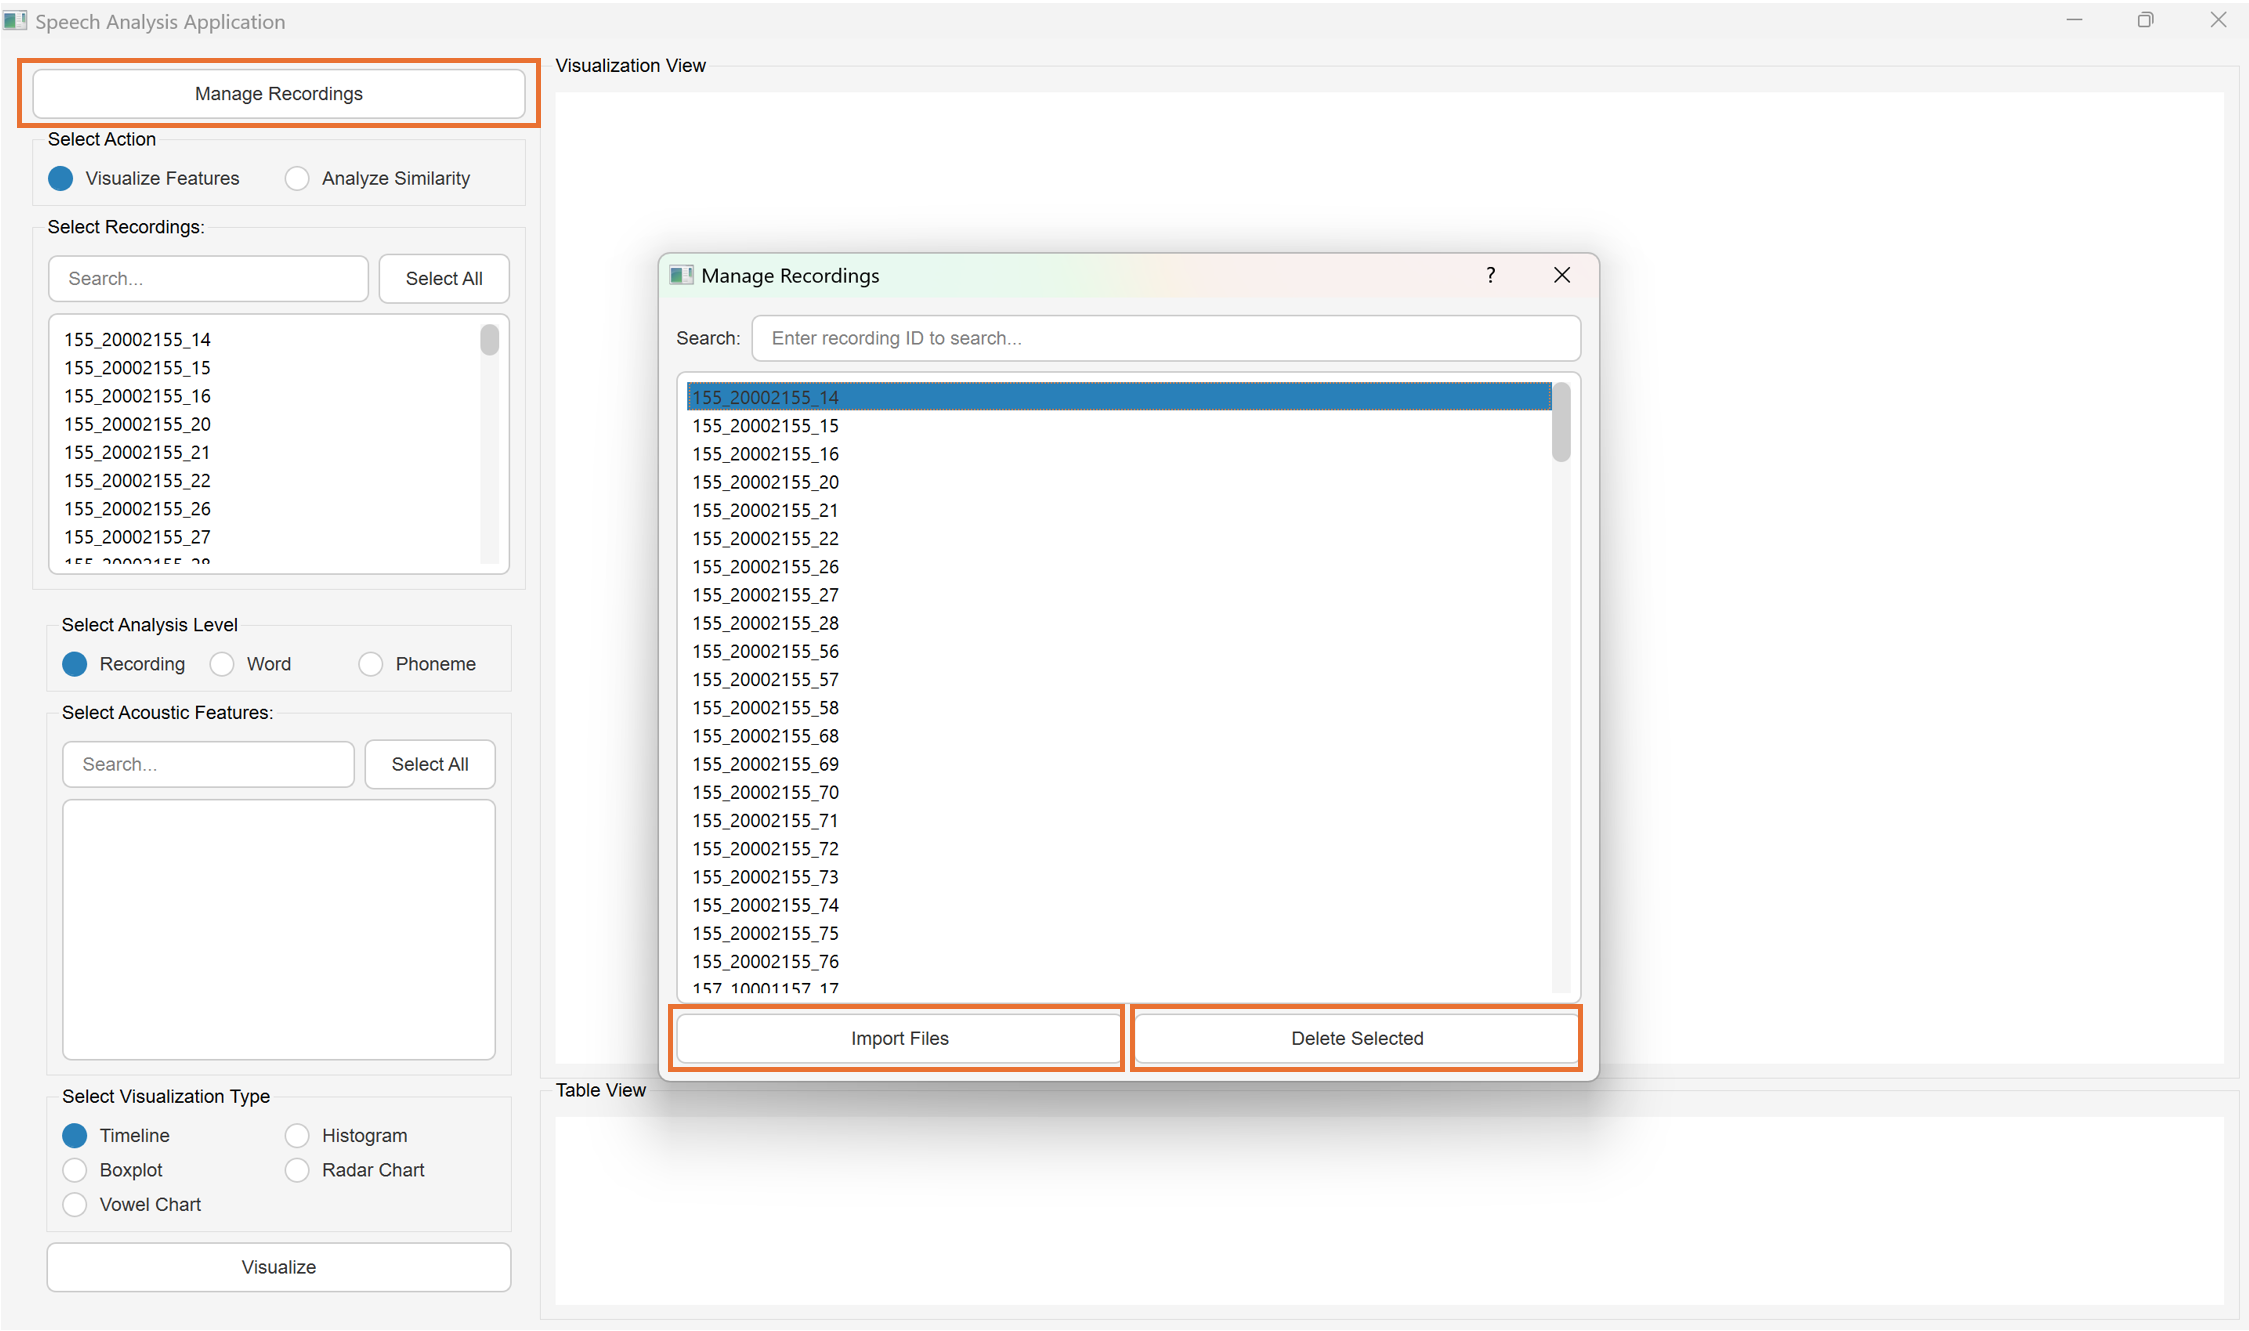
\includegraphics[width=\textwidth]{figures/rakenduse-salvestuste-haldus.png}
    \caption{Rakenduse salvestuste haldus.}
    \label{fig:rakenduse-salvestuste-haldus}
\end{figure}

\textbf{Tunnuste visualiseerimine
}
\begin{itemize}
    \item Visualisatsioonide kuvamiseks kasutaja valib \textit{Visualize Features} valikutest sobivad tunnused.
    \item Valib salvestused (\textit{Select Recordings})
    \item Määrab, kas soovitakse vaadata tunnuseid salvestuse, sõna või foneemi tasandil (\textit{Select Analysis Level}).
    \item Kui valiti foneemi või sõna tasand, tuleb valida ka sõnad või foneemid.
    \item Seejärel valib kasutaja konkreetsed GeMAPS tunnused (\textit{Select Acoustic Feature}s) ning sobiva graafikutüübi (nt ajatelg, karp-, histogramm, radar, vokaalikaart).
    \item Pärast nupule \textit{Visualize} vajutamist, kuvatakse \textit{Visualization View}, kus on: interaktiivne graafik, mille paremas ülanurgas tööriistad (suurendus, pildi eksport jm).
    \item Visualisatsiooni vaate all kuvatakse tabelivaade (\textit{Table View}).
\end{itemize}
Joonisel 3 on näha tunnuse visualiseerimine sõna kohta.
\begin{figure}[H]
    \centering
    \includegraphics[width=\textwidth]{figures/rakenduse-tunnus-sõna-timeline.png}
    \caption{Joondiagrammi näide ühe sõna ja tunnuse visualiseerimisel.}
    \label{fig:rakenduse-tunnus-sõna-timeline.png}
\end{figure}

\textbf{Sarnase kõneleja leidmine}
\begin{itemize}
    \item Kasutaja valib \textit{Analyze Similarity} valiku, määrab salvestused, mida omavahel võrrelda (\textit{Select Recordings}).
    \item See järel Valib ühe (\textit{Target Recording}) salvestuse, millega teisi võrrelda ning sisestab arvu, mitu kõige sarnasemat salvestust soovitakse tulemusena saada (\textit{Number of Similar Items}).
    \item Seejärel valib kasutaja sarnasuse visualiseerimise meetodi: \textit{Cluster Analysis (PCA + KMeans)}, \textit{Feature Similarity Bars} (koosinussarnasus) või \textit{PCA-Based Similarity Bars} (koosinussarnasus PCA ruumis).
    \item Pärast nupuvajutust arvutab rakendus sarnasuse tulemused (nt klasterdamise või koosinussarnasuse), ning kuvatakse \textit{Visualisation View}, kus on: tulpdiagramm, mis näitab salvestuste sarnasuse väärtust või hajuvusdiagramm (klastrite korral), mis eristab klastreid värvidega ning märgib sihtsalvestuse ja kõige sarnasemad salvestused eri sümbolitega.
\end{itemize}

Joonisel 4 on esitatud näide sarnasuse visualiseerimisest PCA ja koosinussarnasuse meetodiga

\begin{figure}[H]
    \centering
    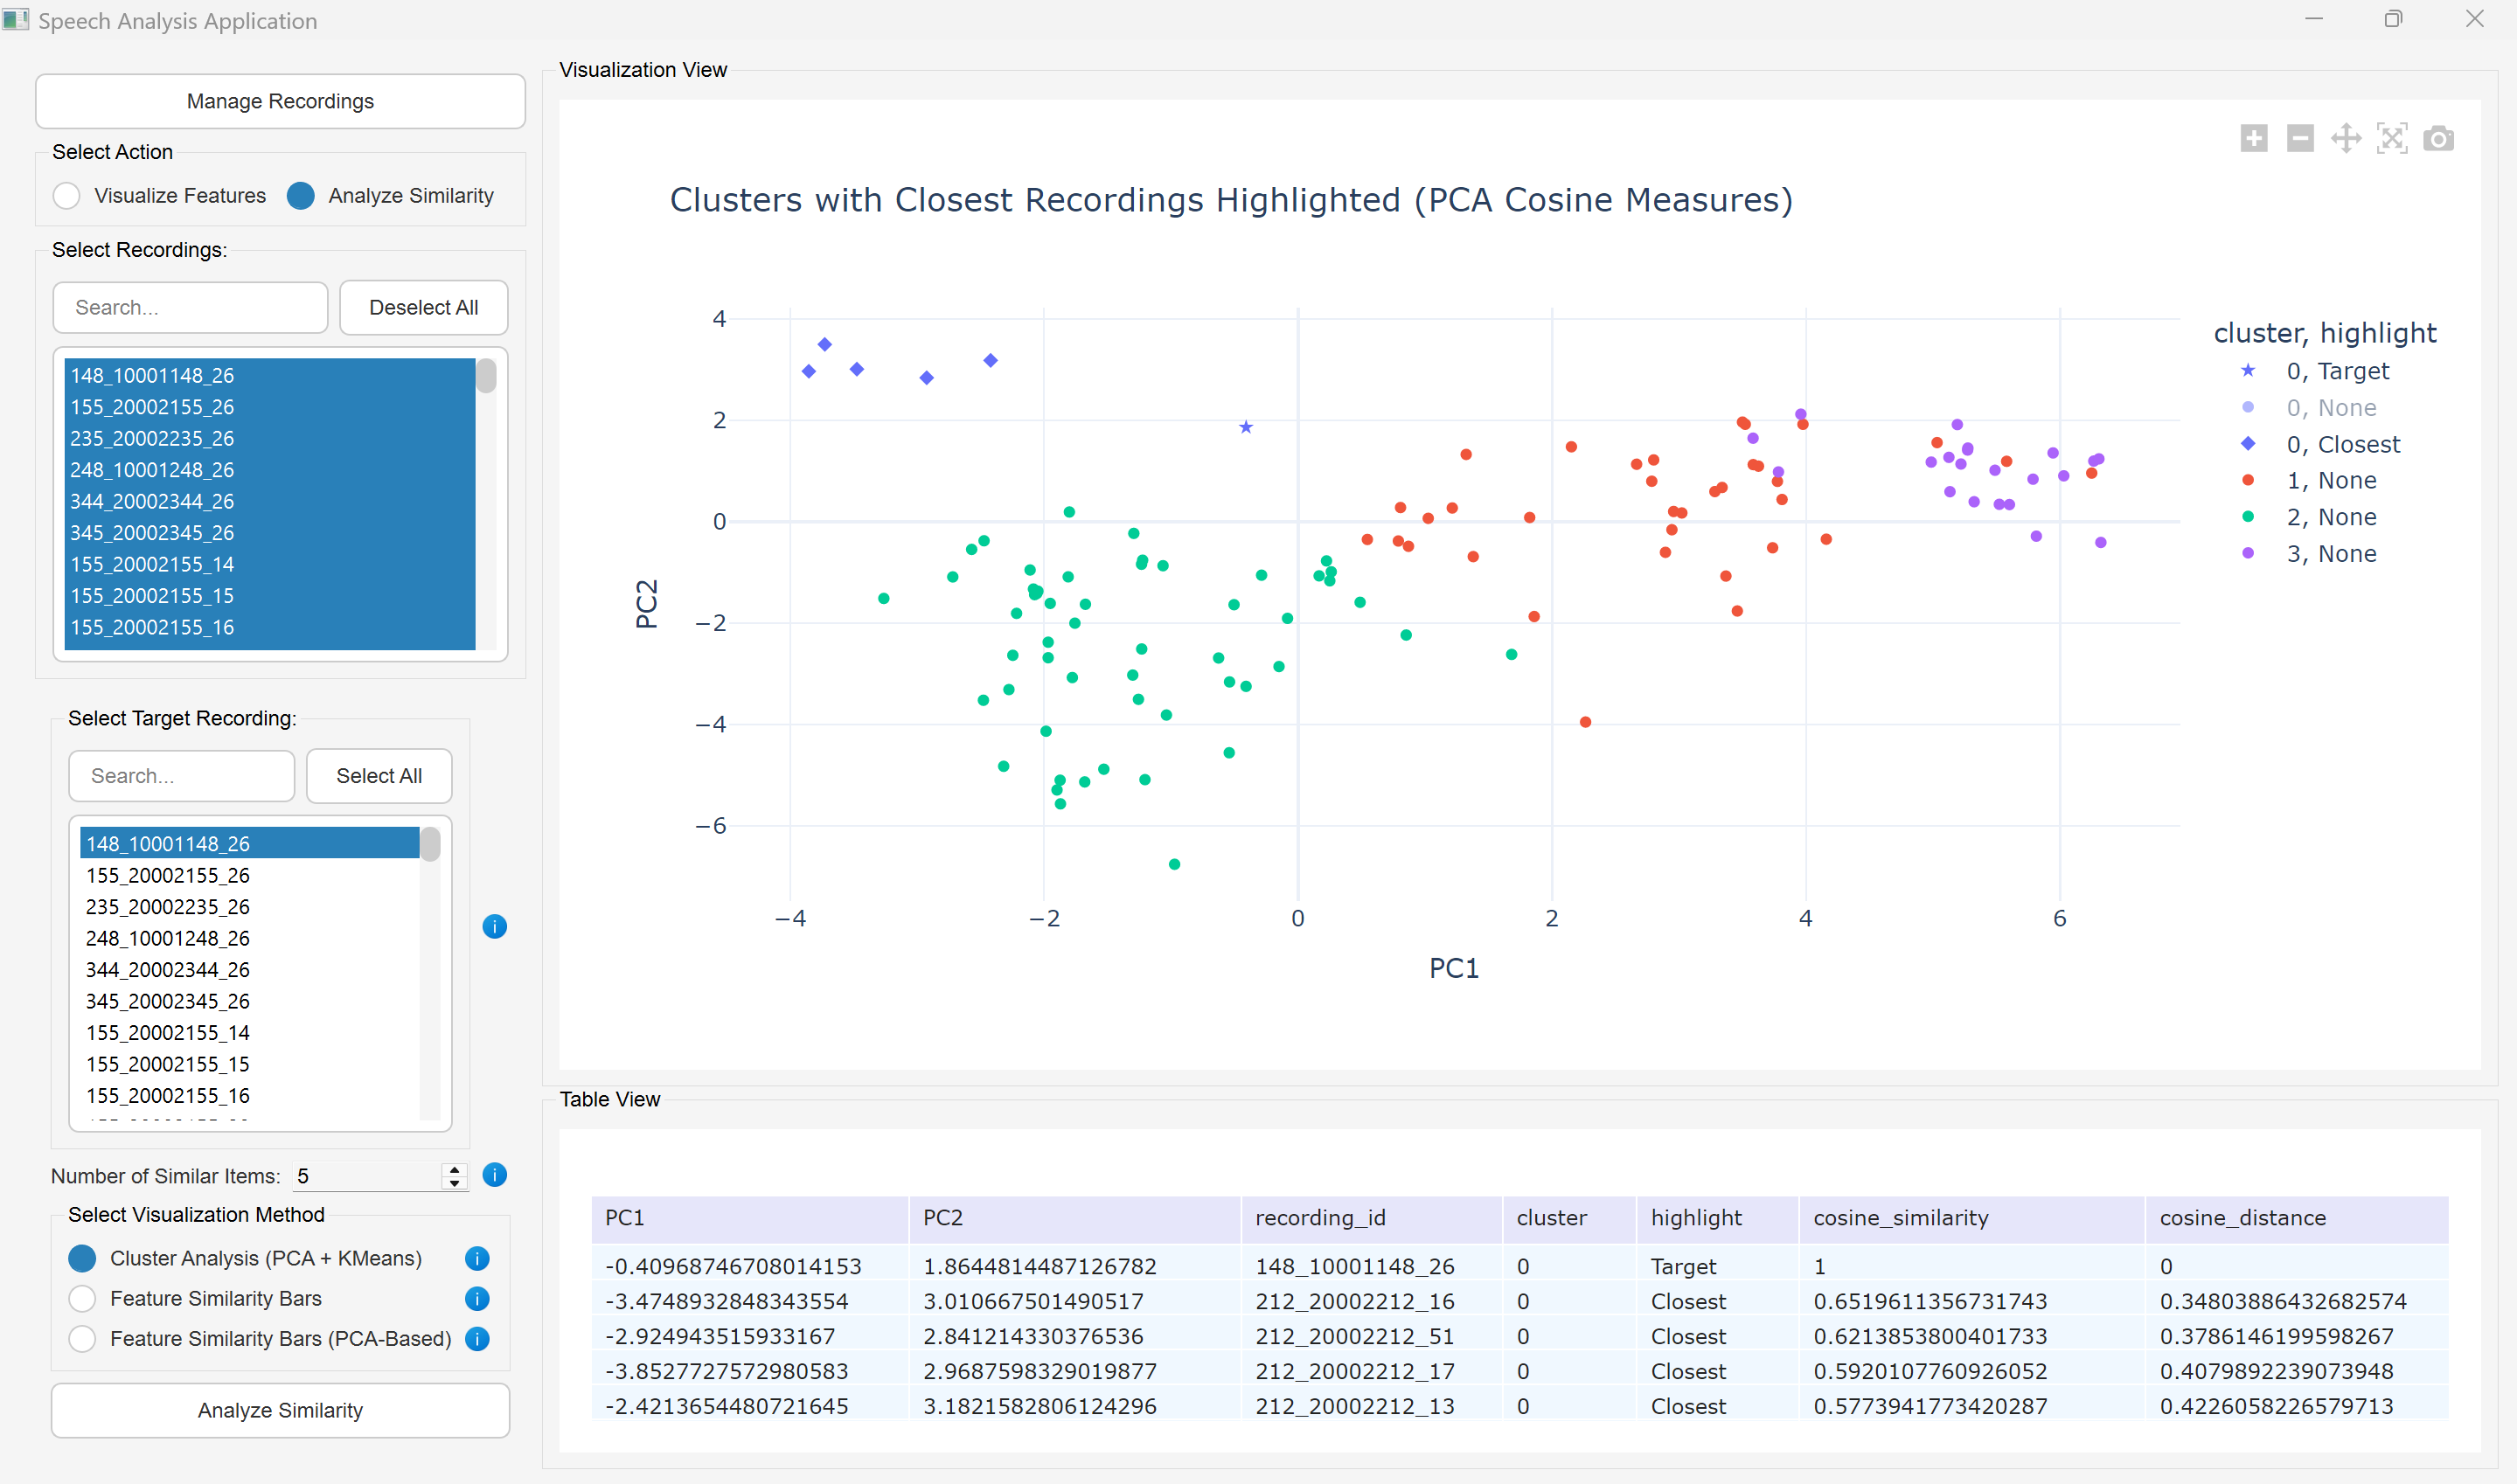
\includegraphics[width=\textwidth]{figures/rakenduse-sarnasus-cluster-closest.png}
    \caption{PCA koosinussarnasuse ja klastrite visualiseerimine hajuvusdiagrammil.}
    \label{fig:rakenduse-sarnasus-cluster-closest}
\end{figure}

\textbf{Helisalvestuse esitamine ja helilaine visualiseerimine}

\begin{itemize}
    \item \textit{Recording Player} sektsioonis kuvatakse rakenduse \textit{data} kaustas asuvad salvestused.
    \item Kasutaja valib faili ning vajutab \textit{Play} nuppu.
    \item Rakendus mängib helisalvestust ning samal ajal kuvatakse helilaine. Mõlemad on kuvatud Joonisel 1.
\end{itemize}

\textbf{Andmete ja visualisatsioonide eksportimine}
\begin{itemize}
    \item Iga valminud graafiku kohal on kaamera märgiga nupp (Plotly sisseehitatud funktsioon). See võimaldab kasutajal salvestada staatilise pildifaili.
    \item Lisaks on juhtpaneelis \textit{Export Graph Data (JSON)} nupp, mis salvestab kasutatud andmed JSON-vormingus. Nupud on nähtaval Joonisel 3.
\end{itemize}

\section{Tulemuse võrdlus olemasoleva lahendusega}
Järgnevalt võrreldakse valminud rakenduse funktsionaalsust Kõneveebi Audiofailide akustiliste omaduste võrdlemise lahendusega (Joonis 5). Kuna see tööriist on alternatiivsetest lahendusest kõige sarnasem oma fookuse, eesmärgi ja funktsionaalsuse poolest. Kuigi Praat või VoiceSauce on palju laiemalt kasutatud akustiliste tunnuste analüüsimisel, on nende fookus ja funktsionaalsus palju laiem ning nad ei keskendu kitsalt eGeMAPS-tunnuste komplektile, nagu Kõneveebi lahendus ja ka loodud rakendus. Seega on sobivam rakendust võrrelda Kõneveebi lahendusega.

\begin{figure}[H]
    \centering
    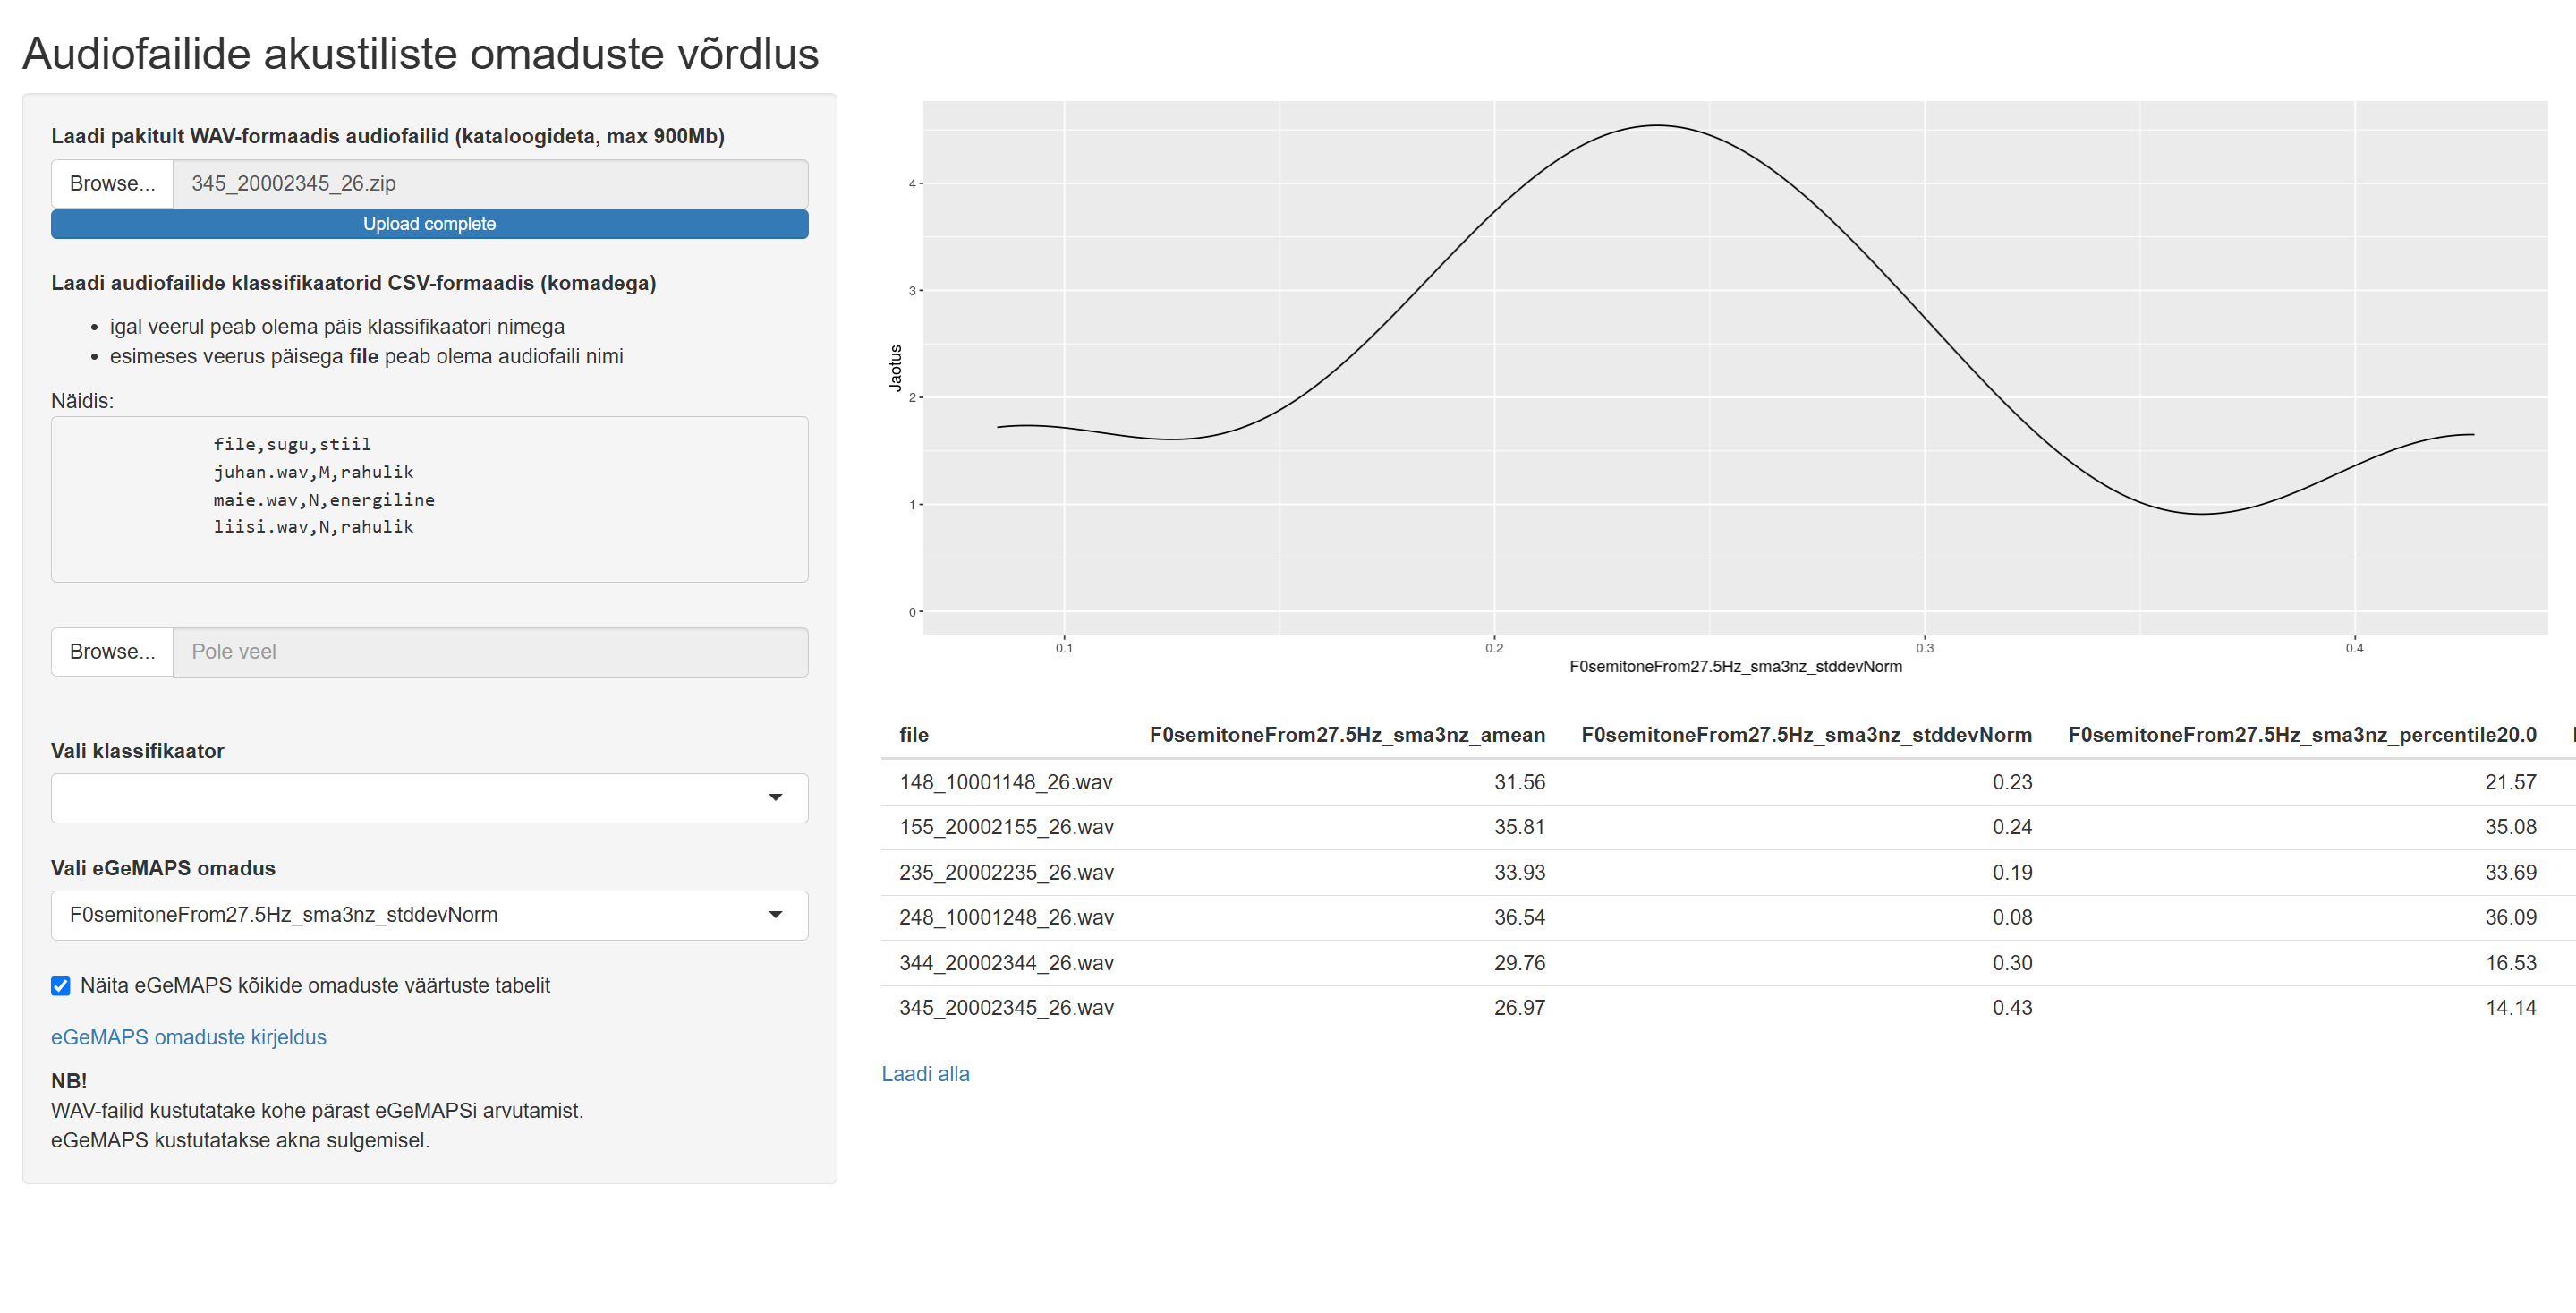
\includegraphics[width=\textwidth]{figures/alt-kõneveeb-põhivaade.png}
    \caption{Kõneveebi Audiofailide akustiliste omaduste võrdlemise rakenduse põhivaade.}
    \label{fig:alt-kõneveeb-põhivaade}
\end{figure}


\begin{longtable}{|p{2.5cm}|p{5.5cm}|p{5.5cm}|}
    \hline
    \textbf{Omadus} & \textbf{Kõneveeb} & \textbf{Loodud rakendus} \\
    \hline
    \endfirsthead
    \hline
    \textbf{Omadus} & \textbf{Kõneveeb} & \textbf{Loodud rakendus} \\
    \hline
    \endhead
    \hline
    \endfoot
    \hline
    \endlastfoot
    
    Tunnuste komplekt &
    Võimaldab analüüsida tervet 88 tunnusega eGeMAPS tunnustekomplekti. &
    Võimaldab analüüsida ainult eGeMAPS v02 LLD komplekti, mis sisaldab üksnes madala taseme deskriptoreid (LLD). \\
    \hline
    
    Rakenduse tüüp &
    Veebirakendus. &
    Installitav töölauarakendus, töötab lokaalselt. \\
    \hline
    
    Kasutajaliides &
    Sarnane põhivaate ülesehitusele nagu loodud rakendusel: juhtpaneel valikutega vasakul ning paremal visualiseerimise ja andmetabeli sektsioonid. &
    Sarnane põhivaate ülesehitusele nagu kõneveebil: juhtpaneel valikutega vasakul ning paremal visualiseerimise ja andmetabeli sektsioonid. \\
    \hline
    
    Erinevate graafikute valik &
    Joondiagramm. &
    Pakub laiemat valikut tunnuste graafikuid, sealhulgas ajatelje diagramm, histogramm, karpdiagramm, radardiagramm, vokaalikaart. Sarnasuse analüüsil on võimalik kasutada hajuv- ja tulpdiagramme. Samuti on graafikud interaktiivsed. \\
    \hline
    
    TexdGridide info kasutamine &
    Ei paku võimalust lugeda ega töödelda TextGrid-failides sisalduvaid ajaintervalle (sõnu, foneeme). Analüüs piirdub salvestuse tasemega. &
    Võimaldab lugeda TextGrid-faili, seostada konkreetsete tunnuste väärtusi sõna või foneemi ajaintervalliga ning seejärel kuvada eraldi vaateid/visualiseeringuid valitud segmentidele. \\
    \hline
    
    Sarnaste salvestuste leidmine &
    Puudub. &
    Võimaldab mitut sarnasuse arvutamise meetodit (klasterdamine, koosinussarnasus, PCA-järgne koosinussarnasus). Visualiseerib tulemused kas tulpdiagrammina (näiteks kõige sarnasemad salvestised) või hajuvusdiagrammil, kus sihtsalvestis ja sarnased salvestised on esile tõstetud. \\
    \hline
    
    Andmete eksport &
    On nupp arvutatud tunnuste andmete allalaadimiseks, kuid see ei toiminud antud töö kirjutamise ajal. &
    Toetab andmete eksporti JSON faili ja pildifaili kujul. \\
    \hline
    
    Andmete haldus &
    Üleslaetud failid ja arvutatud tunnused kustutatakse seansi lõpus. Failide maht on piiratud (kuni 900 MB) ja tulemusi ei salvestata. &
    Kasutab MongoDB andmebaasi analüüsi andmete hoidmiseks. \\
    \hline

\end{longtable}

Kokkuvõttes on Kõneveebi rakendusel ja loodud rakendusel sarnane põhifookus, kuid veidi erinev ulatus. Kõneveeb on kindlasti mugav ja kiirem, kuna see ei vaja eraldi installeerimist ja seadistamist. Kuid käesolev rakendus on laiema funktsionaalsusega ning sobib paremini mahukamaks analüüsiks, kus on vaja erinevaid visualiseerimise meetodeid, analüüsitulemuste salvestamist ja sarnasuse analüüsi.

\section{Tagasiside}
Rakenduse valideerimiseks küsiti tagasisidet ühelt foneetikauurijalt, kellele saadeti rakenduse installeritav versioon koos kasutusjuhendiga ja tagasiside küsimustega, mis on esitatud Lisas 4.

\textbf{Rakenduse graafikute arusaadavus ja kasulikkus}. Testija tagaside oli, et rakenduses loodud graafikud olid üldiselt arusaadavad ning märgiti, et need võiksid olla mugavad kiireks analüüsiks. Kõige kasulikumaks visualisatsiooniks peeti vokaalikaarti.

\textbf{Tehnilised probleemid ja tõrked}.
Tagasiside põhjal ei märgatud rakenduse kasutamise ajal tehnilisi probleeme ega tõrkeid

\textbf{Kasutajasõbralikkuse hinnang}.
Kasutajasõbralikkuse ja mugavuse osas anti rakendusele hinnang 3 skaalal 1-5, kus 1="väga mugav" ja 5="väga ebamugav". Kuigi rakendus ei olnud kasutaja arvates väga ebamugav, mainiti, et mõned klikkimisega seotud iseärasused vajasid harjumist.

Näiteks tekitas segadust, et histogrammi visualisatsiooni valik muutub mitte-aktiivseks, kui on valitud korraga üle kahe tunnuse ja salvestuse korraga. See oli tahtlik piirang, et vältida olukordi, kus liiga paljude tunnuste ja salvestuste samaaegne kuvamine ühel graafikul muudaks tulemused raskesti loetavaks. Selle piirangu oleks pidanud kasutajale arusaadavamaks tegema näiteks teavituste või infonuppude abil, nagu tehti paljude rakenduse teiste funktsioonide puhu, kuid kahjuks jäid need selle piirangu jaoks lisamata.

\section{Võimalused edasiarenduseks}
Rakendusel on palju võimalusi edasiarendusteks. Järgmiselt tuuakse välja mõned võimalused, mis tulid esile peale arenduse lõppu:
\begin{itemize}
    \item Võimaldada erinevate GeMAPS tunnustekomplektide arvutamine
    \item Võimaldada erinevate normaliseerimismeetodite rakendamine ja mitte rakendamine, et kasutajal oleks rohkem kontrolli andmete visualiseerimisel. Näiteks vokaalikaardi puhul normaliseeritakse väärtused Lobanov meetodiga ja ei ole võimalust teisi meetodeid kasutada või väärtused normaliseerimata jätta.
    \item Kasutajaliidese mugavdamine: näiteks menüüs võiks olla rohkem ruumi tunnuste ja salvestuste valimiseks
    \item Sarnasuse analüüsi valideerimine, rohkem meetodeid sarnaste salvestuste leidmiseks
    \item Andmete mahu probleemi lahendamine: kui andmete hulk kasvab, muutub rakendus aeglasemaks
    \item Muuta rakendus lihtsamini installeeritavaks, et kasutaja ei peaks MongoDB andmebaasi seadistama.
\end{itemize}

Lisaks tõi foneetikauurija tagasisides esile järgmised soovitused:
\begin{itemize}
    \item Lisada funktsioon helifailide lõikamiseks.
    \item Luua võimalus esitada helifaile otse failide valiku menüüst.
    \item Kuvada rakenduses rohkem arvandmeid.
\end{itemize}


\chapter{Kokkuvõte}\label{chapter:summary} 
\input{chapters/6. Kokkuvõte}
